\documentclass[a4paper, oneside, 11pt]{article}
\usepackage{graphicx} % Required for inserting images

\usepackage[margin=2cm]{geometry}
\usepackage[style=ieee]{biblatex}
\addbibresource{references.bib}

\title{Using Machine Learning to Identify Positions in Grappling}
\author{Talhaa Hussain}
\date{}
\begin{document}

\maketitle


\begin{abstract}
    Grappling is a form of unarmed combat that doesn't involve strikes (i.e. punches, kicks, knees, elbows or headbutts), and instead revolves around takedowns, ground control and submission holds. There are many variants of grappling, but generally the objectives are the same - to either pin an opponent to the ground and prevent them from moving, or to cause them to concede/submit, either through a choke/stranglehold or through a joint lock.

    Unlike striking, grappling is much more complex due to the range of techniques, positions, submissions and holds available. This can make identifying positions and techniques (either when learning or officiating a grappling match) quite difficult. This project aims to use machine learning and computer vision to identify different positions in grappling, outline and build a solution, and provide a timeline for the development of the solution. Machine learning techniques has been shown to be capable of identifying and distinguishing different positions and patterns of the human body, such as faces, hands or posture. This paper explores existing solutions to similar problems, and outlines some basic concepts regarding human pose estimation (HPE) and deep learning, which have seen rapid growth and development over the last decade. 
\end{abstract}


\newpage
\section{Introduction}

Grappling is a form of unarmed combat that doesn't involve strikes (i.e. punches or kicks), and instead revolves around takedowns, ground control and submission holds \cite{ribeiro2008jiu}. There are many variants of grappling \cite{cejudo2012wrestling}\cite{DifferentTypesOfWrestling}, but generally the objectives are the same - to either pin an opponent to the ground (often after performing a throw) and prevent them from moving \cite{cejudo2012wrestling}, or to cause them to concede/submit, either through a choke/stranglehold or through a joint lock \cite{takagaki2012techniques}. Grappling arts are constantly evolving, with new strategies and approaches constantly emerging \cite{JohnDanaherJiuJitsuEvolution}.

Within grappling, there are a wide range of positions, some of which are neutral, others providing some advantage to one grappler or the other. In all forms of grappling, the more advantageous fighter is usually the one with superior control of their opponent \cite{ribeiro2008jiu}, as shown in Figure \ref{fig:grapplingpositions}.


\begin{figure}[h]
    \centering
    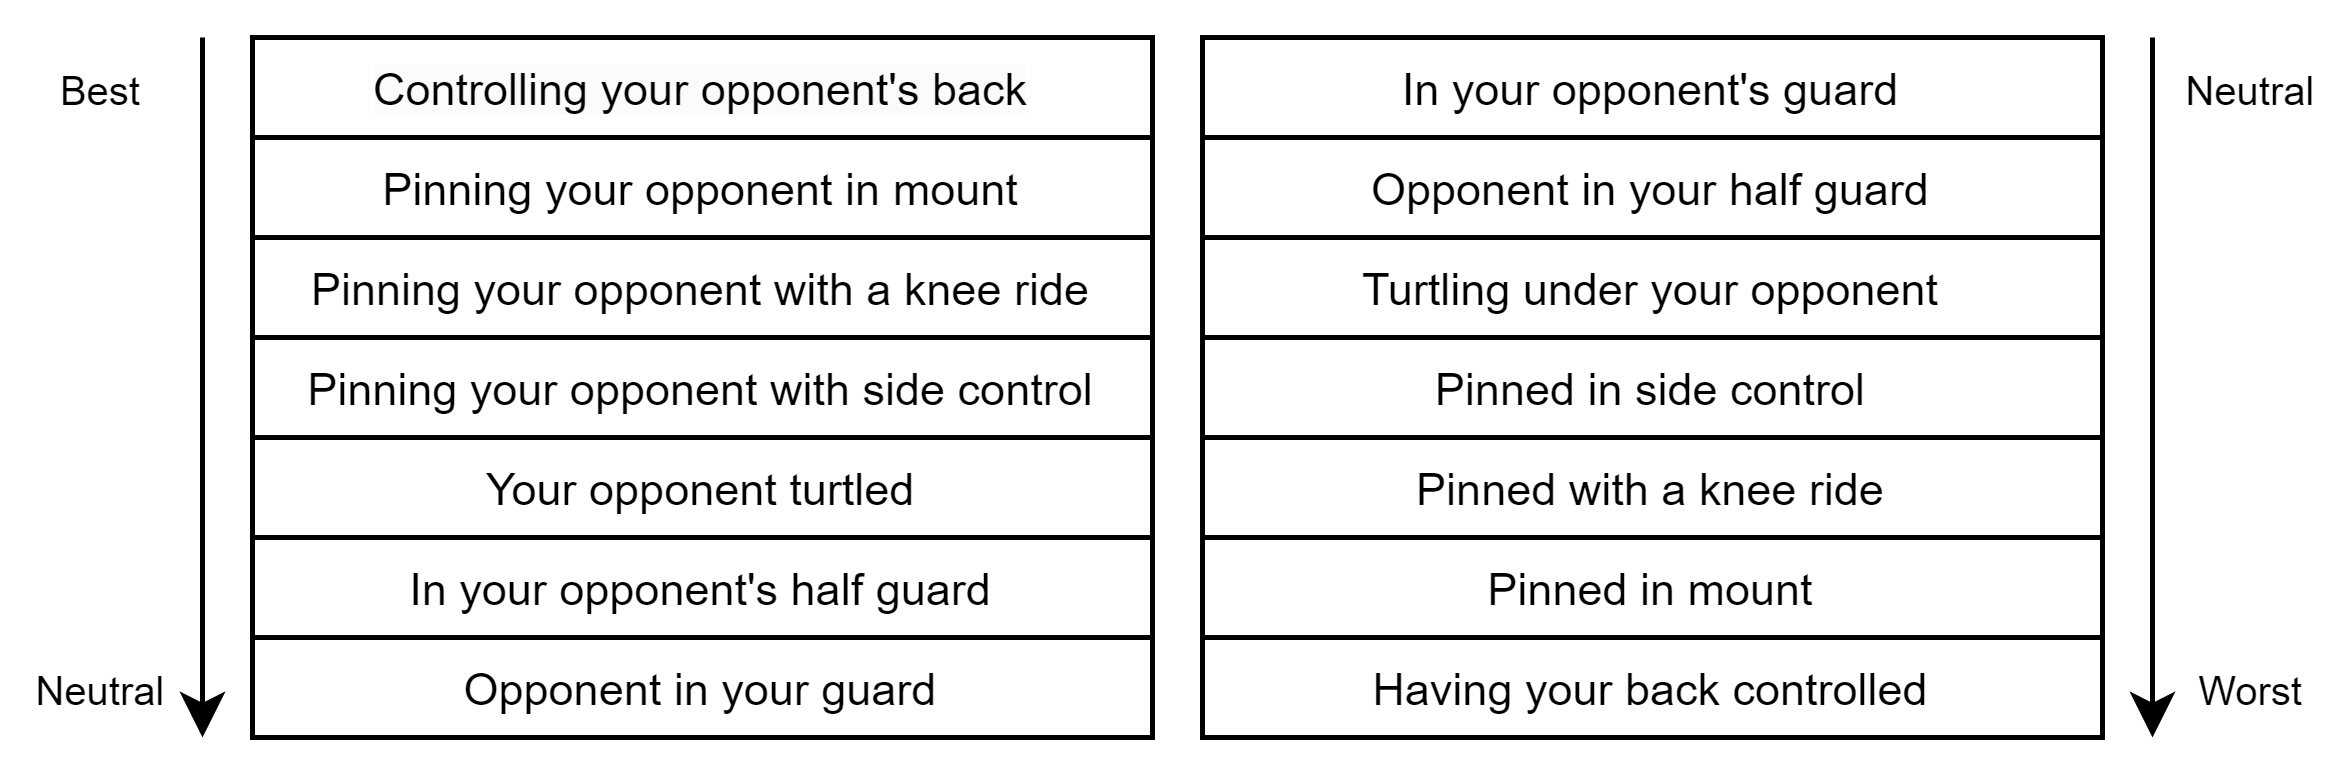
\includegraphics[scale = 0.15]{img/Grappling positions.drawio (1).png}
    \caption{Positional hierarchy in ground submission grappling}
    \label{fig:grapplingpositions}
\end{figure}

Because of the competitive and fast nature of grappling, it can often be hard to identify different positions in an encounter. Often in competition, competitors are awarded points on gaining positional advantages or landing throws/take downs; referees and judges are relied upon for tallying scores and awarding points when needed. However, this has been unreliable in the past, with referees making poor calls and making mistakes, not identifying positions or awarding competitors correctly for throws or pins. Furthermore, with the emergence of online videos, it can be hard for the average viewer or student to understand and distinguish what's going on in a video of an intense match - the rapid transitioning and movement between positions can be very confusing and some positions may be mistaken for another.

Computer vision is a rapidly evolving field of artificial intelligence that looks to enable computers to "see", allowing them to identify and distinguish objects \cite{DefineComputerVision}. Machine learning is another branch of artificial intelligence, and involves "teaching" computers to learn from some data, such as images or statistics \cite{nielsen2015neural}. Deep learning is a specific subset of machine learning methods, specifically built around neural networks with certain characteristics \cite{nielsen2015neural}. Deep learning techniques work extremely well with computer vision techniques \cite{ComputerVisionAndDeepLearning}, and both computer vision and deep learning can be applied to the problem at hand. Computer vision gives rise to human pose estimation, the recognition and identification of different poses and positions \cite{DefineHumanPoseEstimation}. This can be applied to identify positions and techniques seen in grappling, while deep learning can enable a system to classify detected techniques. This project intends to use these concepts of computer vision (specifically pose recognition) and deep learning techniques to identify various grappling positions in both stand-up fighting and ground-fighting.


\section{Literature Review}

This section outlines key concepts in this project and looks at previous works on related problems.

\subsection{Perceptrons, Neural Networks and Deep Learning}

Neural networks are structures that enable deep learning to take place. They're based off of the animal brain, composed of perceptrons and connections between these perceptrons (similar to neurons and their connections). Perceptrons are single units, the smallest constituent part of a neural network. Perceptrons take a number of binary inputs, and produce a single binary output based on the inputs. Each input has a weight associated with it, a real number that expresses the importance of the input.

\begin{figure}[ht]
    \centering
    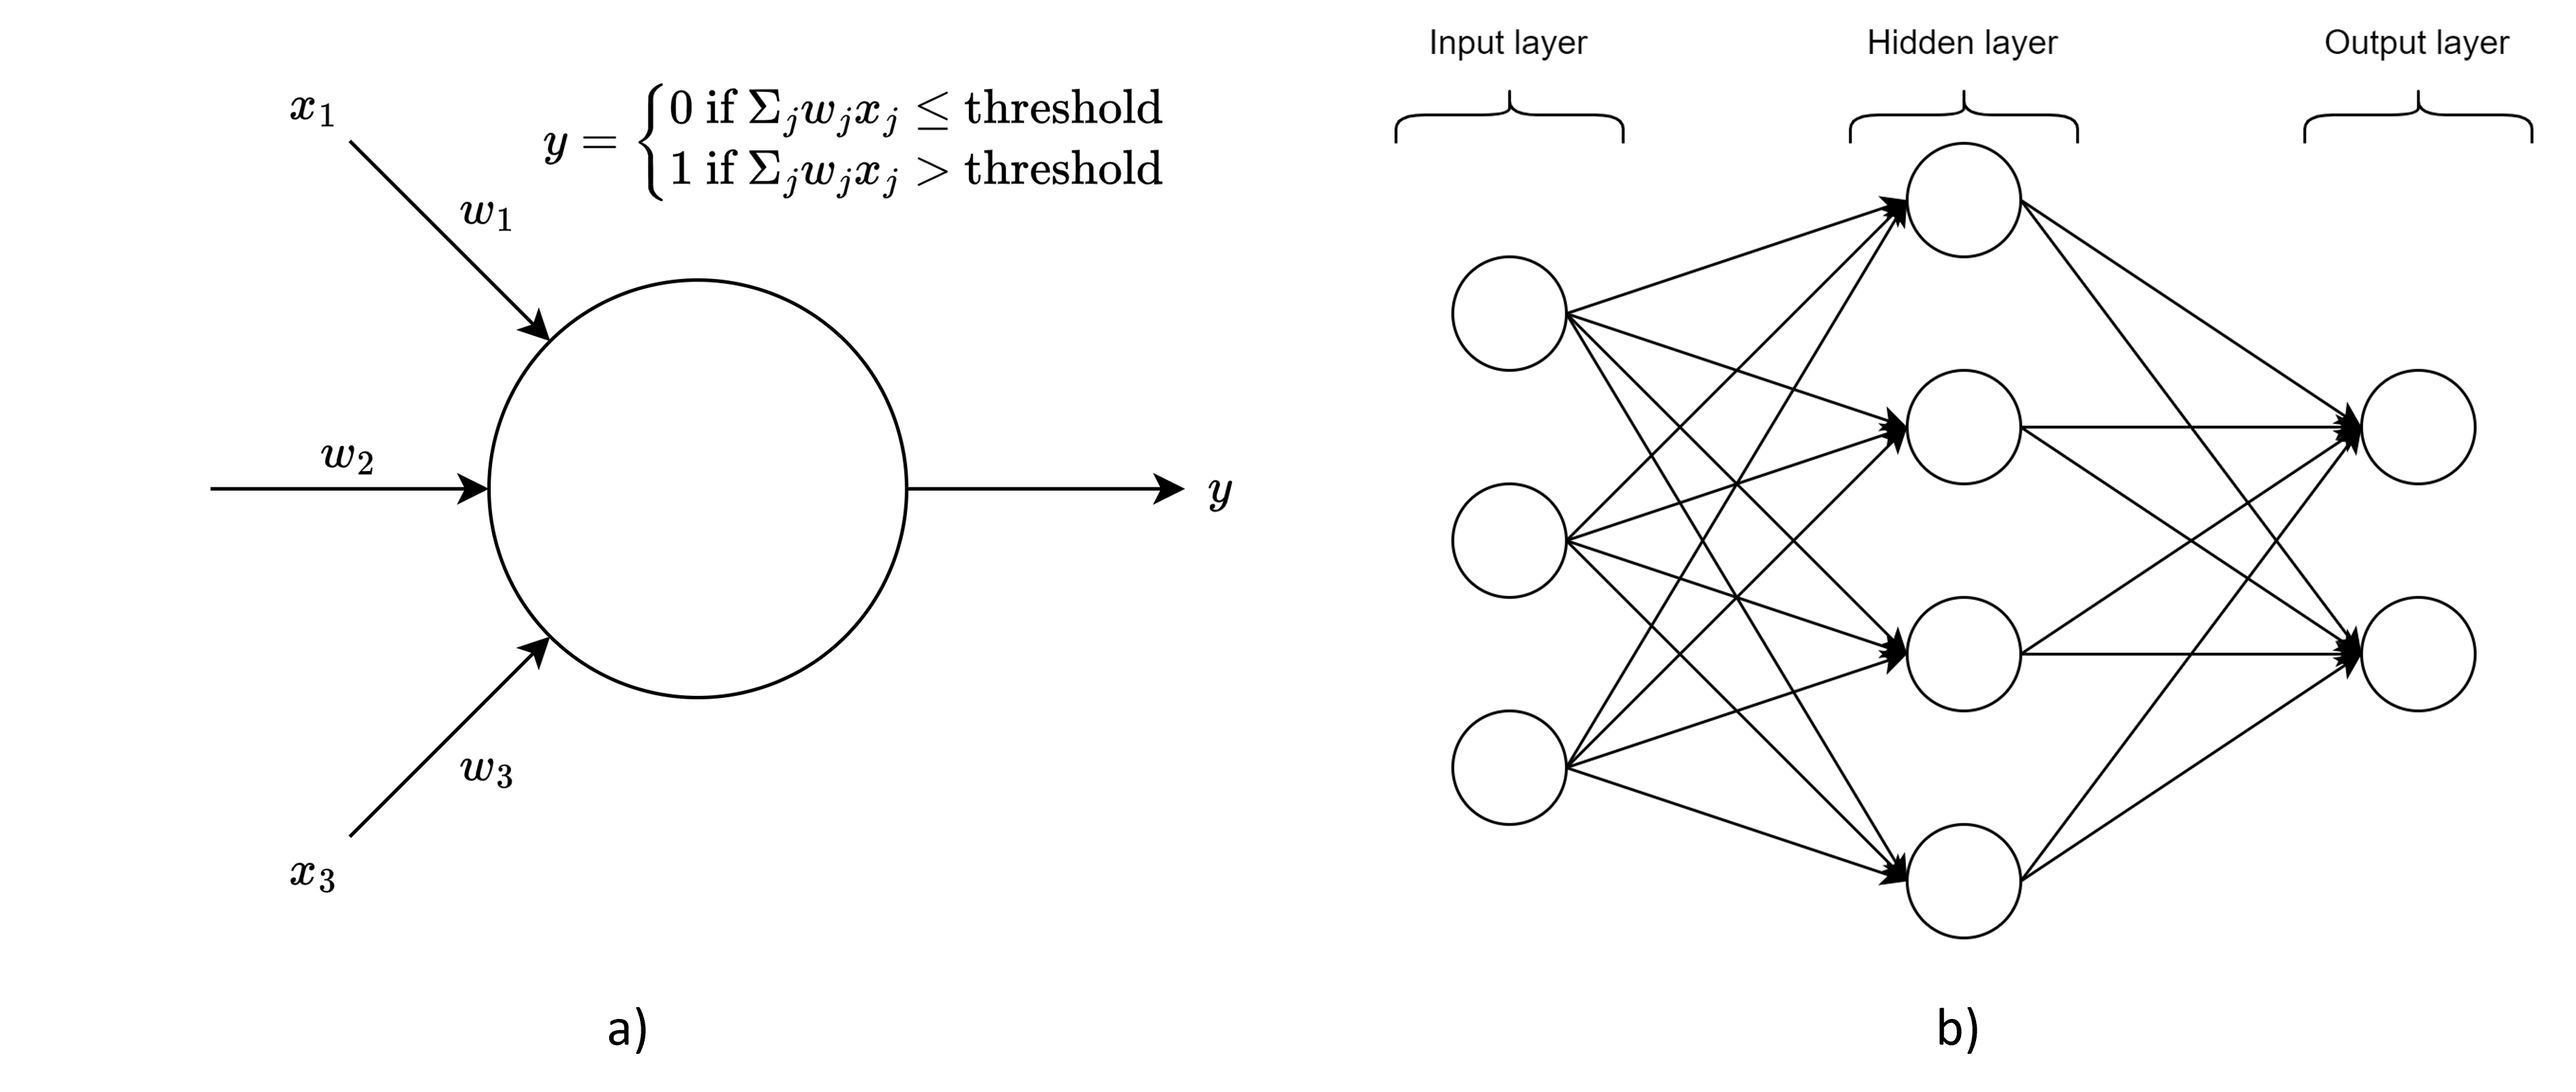
\includegraphics[scale = 0.5]{img/neurals combined.png}
    \caption{a) A perceptron. b) A neural network. Please note that all perceptrons have a single output; the multiple arrows coming out of a perceptron are the same output repeated many times over.}
    \label{fig:unifiedneural}
\end{figure}

As shown above in Figure \ref{fig:unifiedneural}a), $y$ is 1 if and only if the weighted sum $\Sigma_jw_jx_j$ is greater than some threshold value; otherwise, the output $y$ is 0. By composing perceptrons into layers (columns), where the output of perceptrons in layer $n$ become the input to the perceptrons in layer $n + 1$, we have the basic model of a neural network, as shown above in Figure \ref{fig:unifiedneural}b).

In a basic neural network, perceptrons in a layer never receive input or output from each other. As aforementioned, the structure is inspired by the animal brain, a literal network of neurons. Using neural networks, we can simulate learning and decision making. The layer between the input and output layers is known as the hidden layer. Instead of one hidden layer, we can have several - these are called deep neural networks \cite{nielsen2015neural}. Deep learning is heavily inspired by the human brain. The idea behind deep learning (specifically in image recognition) is the fact that deep learning methods automatically extract features from the input image. In image recognition, feature extraction is when specific (important) parts of an image are extracted, to allow the image to be understood, recognised or classified. Unlike traditional machine learning methods, where feature extraction has to be done manually, deep learning models allow for feature extraction to take place automatically, due to the additional hidden layers in the network.

Transformers and CNNs (Convolutional Neural Networks) are two deep learning architectures that are currently at the forefront of computer vision and image recognition. Transformers, introduced in 2017 \cite{TransformersIntro}, are extremely popular among recent human pose recognition software \cite{xu2022vitpose}, while convolutional neural networks have been historically shown to be effective with recognising patterns in images and specifying these patterns \cite{nielsen2015neural}. 

\subsection{Data-set Augmentation}

When working with images, it's possible to augment the data-set to increase its size. Data-set augmentation (in the context of images) involves taking the original data and making some changes, and adding these modified images into the data-set \cite{devries2017dataset}. For example, we may take an image and flip it, crop it, adjust the brightness, recolour it, etc.

The benefit of data-set augmentation is that it introduces diversity into the data-set \cite{devries2017dataset}. It also improves the accuracy of the model being trained. In this specific instance, when recognising grappling positions using deep learning and HPE, data-set augmentation is a clear benefit, because it enables the trained model to work well with images of a variety of resolutions, sizes, and colour grades. This means the software could potentially be used to analyse competitions from a variety of sources, including historical bouts.

\subsection{Human Pose Estimation}

Human pose estimation is a major field within computer vision, and has many applications in the real world. Human pose estimation aims to identify and track key points on a human individual, usually limbs and joints, to determine the orientation and pose of the subject \cite{DefineHumanPoseEstimation}. There are two approaches with to pose estimation - top-down and bottom-up. Top-down methods first identify a human individual in an image, forming a bounding box around them, before trying to identify human joints or other points of interest within the bounding box \cite{HPEVisoAI} \cite{HPEDeepLearningMethods}. Bottom-up approaches identify all joints or points of interest on an image first, before trying to group them together to form a human body \cite{HPEDeepLearningMethods}. Top-down methods suffer when there are many people in the input image \cite{HPEDeepLearningMethods}; the computation cost grows due to the need to identify and draw more bounding boxes. Contrarily, bottom-up methods remain stable even as the number of people in the image grows \cite{HPEDeepLearningMethods}. However, in the case where individuals in the image overlap, bottom-up methods struggle to group body parts to the individual to whom they belong to \cite{HPEDeepLearningMethods}. 

There are two main types of HPE - 2D pose estimation and 3D pose estimation \cite{HumanPose2dvs3d}. 2D pose estimation is concerned with the position of a subject within a 2D space; 3D pose estimation includes an extra z-axis to the position of limbs/joints, predicting the position of the subject in a 3-dimensional space. While 2D HPE tends to be easier to implement and faster \cite{HPEFitnessRehab} \cite{HumanPose2dvs3d}, 3D HPE yields a higher accuracy because it takes into account the third dimension of space \cite{HPEFitnessRehab}.

\begin{figure}[ht]
    \centering
    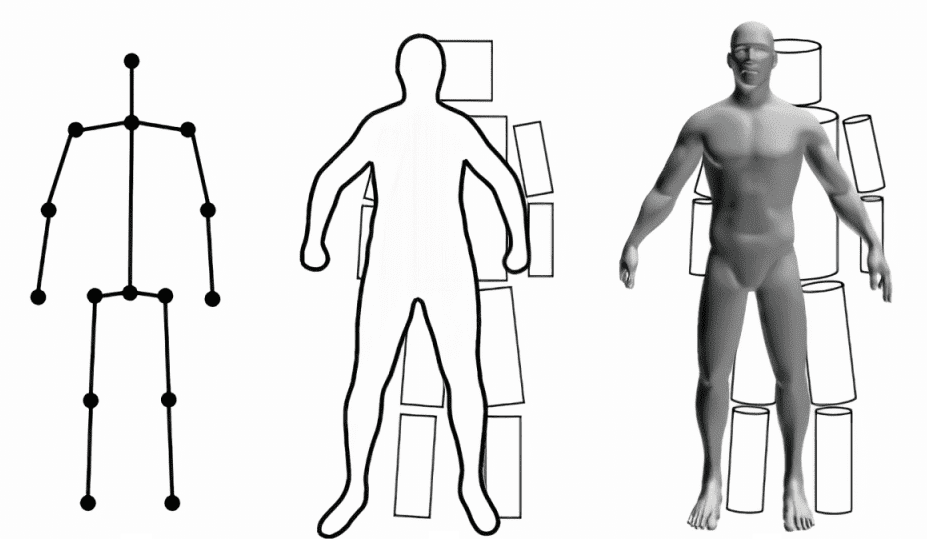
\includegraphics[scale = 0.26]{img/humanbodymodels.png}
    \caption{HPE models. From left to right: kinematic model, planar model, volumetric model \cite{HPEDeepLearningMethods}.}
    \label{fig:humanbodymodels}
\end{figure}

With regards to the human models, there are three main types - a kinematic model, a planar (contour-based) model and a volumetric model, each with varying degrees of detail with regards to visualising the human body \cite{HPEFitnessRehab}\cite{HPEDeepLearningMethods}\cite{HPEVisoAI}, as shown above in Figure \ref{fig:humanbodymodels}. Kinematic (skeleton-based models) models represent the human body through a set of joint positions and limb orientations. They are used for 2D and 3D pose estimation. Planar (contour-based) models represent the shape of the human body through 2D polygons as an outline \cite{HPEVisoAI}\cite{HPEDeepLearningMethods}. Planar models are used for 2D pose estimation only. Volumetric models are the most detailed of the three, employing a full 3D model of the human body \cite{HPEDeepLearningMethods}. These are used exclusively for 3D pose estimation \cite{HPEVisoAI}. Generally, kinematic models are the most popular, because they are simple and easy to implement, and can be used in 2D and 3D HPE \cite{HPEFitnessRehab}\cite{HPEUltimateGuide}.


\subsection{Grappling and Wrestling}

This subsection aims to disambiguate the basic concepts of grappling.
Wrestling is a subset of grappling that revolves around attempting to pin the opponent to the ground. This is not to be confused with professional wrestling, a form of athletic theatre, with popular promotions such as the WWE (World Wrestling Entertainment). There are many forms of wrestling with different rule-sets, but in general, the objectives remain the same - obtain a positional advantage over the opponent by controlling them, throwing them, pinning them and (under some rulesets) submitting them. 

The two variants of wrestling contested at the Olympics (not including Judo, which is discussed later) are freestyle wrestling and Greco-Roman wrestling. They both have the same objective - pin the opponent onto their back such that both shoulder blades touch the ground simultaneously. Wrestlers throw each other in order to achieve this. The key difference between Greco-Roman and freestyle is that in Greco-Roman, a wrestler is not allowed to attack below the waist or use their legs in any way. Neither freestyle nor Greco-Roman wrestling allow submissions.

Judo is a Japanese martial art, and is a form of wrestling and an Olympic sport. Judo players, called Judoka, wear a traditional Japanese jacket called a kimono, or a gi. Judoka aim to score an "ippon", which is a full score, ending the match immediately and winning. The four ways to potentially score an ippon (winning score) are by:
\begin{itemize}
    \item Throwing your opponent onto their back with force, speed and control
    \item Pinning your opponent's shoulder blades to the ground for 20 seconds by holding their torso
    \item Forcing a submission by armlock
    \item Forcing a submission by choke/strangulation
\end{itemize}

Brazilian Jiu-jitsu, also known more simply as BJJ or Jiu-jitsu, is a martial art and grappling combat sport. Unlike Judo or Olympic wrestling, BJJ is focused very heavily on ground-based grappling, with a reduced focus on stand-up grappling. The objective of BJJ is to gain a positional advantage over your opponent, and eventually submit them. There are some key differences between Jiu-jitsu and the other styles previously mentioned -BJJ can be contested in the Gi or without the Gi (also known as No Gi Jiu-jitsu). BJJ also allows for a much wider range of submissions than Judo (for example, Judo does not permit leglocks, whereas Jiu-jitsu does). Unlike any of the other styles mentioned, BJJ does not have pins as a win condition. An opponent can be pinned with their shoulder blades on the ground, but this will not end the bout. BJJ has a much greater emphasis on "guard-play", which is when a player on the bottom position uses their legs to control their opponent.

\begin{figure}[ht]
    \centering
    \includegraphics[scale = 0.45]{img/combat sports.png}
    \caption{(From top-left, clockwise) A wrestler pins their opponent; a Judoka attempting a throw; a player holds their opponent in closed guard (Gi BJJ); a player attempts to pass their opponent's open guard (No-Gi BJJ).}
    \label{fig:bjjguard}
\end{figure}

While there are many variants of grappling and rulesets, in general, all grappling arts follow the same principles: takedown, pin, control, submit. The aim of this project is to create a general algorithm for recognising universal grappling positions, not bound or limited by any particular ruleset. 

This algorithm can then be applied to any grappling sport, ruleset or even MMA (mixed martial arts) to give some insight and information about the current position in the bout.

\subsection{Current Programs and Solutions}

Initially, the focus was on finding current solutions to human pose estimation problems with regards to marital arts in general. Karate seems to be the most widely researched martial art, with papers \cite{KarateCombatPunchAnticipationBJJPaper} \cite{KarateKata} \cite{PsychomotorPerformanceKarateCombatBJJPaper} \cite{OpenPoseMAPresentationBJJPaper} all concerning computer vision research surrounding Karate. The 2023 paper "Real-time Detection of Taikyoku Shodan Karate Kata Poses Using Classical Machine Learning and Deep Learning Models" \cite{KarateKata} by M. Walid, M. Ameen and A. Atia uses machine learning and deep learning models to enable HPE in real-time. The paper focused on the Karate kata (form) "Taikyoku Shodan", detecting different poses throughout the kata. The researchers employed various classical machine learning methods and deep learning methods, and analysed their performance. The researchers found that the most accurate method was the Random Forest, a classical ML method, which achieved an accuracy of 98\% \cite{KarateKata}. The most accurate deep learning method tested was the Long-Short term memory model, achieving an accuracy of 97\% \cite{KarateKata}.

While in this instance, a classical ML method did indeed achieve a higher success rate than a deep learning method, it's worth noting that the researchers in this instance were focused on analysing Karate kata, particularly Taikyoku Shodan, a kata that is known for its simplicity, comprising of only two techniques, all performed in one stance \cite{taikyoku1}\cite{taikyoku2}. Taikyoku is generally one of the first kata taught to beginners in Shotokan Karate \cite{taikyoku1}\cite{taikyoku3}, and is only constituent of 20 sequential moves \cite{KarateKata}\cite{taikyoku1}. Compared to grappling, where there are two individuals engaging in rapid and complicated combat, with many complex positions, it's apparent that while both problems are focused around identifying positions in martial arts, they are still vastly different. As a result, the results of this paper are not fully applicable in the context of identifying positions in grappling. In the 2018 paper "Deep Learning for Computer Vision: A Brief Review" by A. Voulodimos, N. Doulamis, A. Doulamis and E. Protopapadakis, it is stated that in recent years, deep learning methods have outperformed machine learning techniques in computer vision \cite{ComputerVisionAndDeepLearning}. With regards to human pose estimation, in recent years, all cutting edge approaches to HPE have been based on deep learning \cite{IdentifyingBJJPositions}. While the recent paper by M. Walid et al. isn't completely invalid or redundant, in order to find more relatable existing solutions to the problem at hand, the focus should be on solutions focused on HPE with regards to grappling martial arts between two combatants, rather than martial arts in general.

The 2022 paper "Video-Based Detection of Combat Positions and Automatic Scoring in Jiu-jitsu" by V. Hudovernik and D. Skočaj \cite{IdentifyingBJJPositions} fit this criteria exactly - the paper was concerned with identifying the various positions in Brazilian Jiu-jitsu, one of the main three grappling arts presented in this problem. In this paper, a pipeline was proposed  with three main outputs: (i) tracking the poses of both competitors, (ii) classification of combat positions at each frame (under a BJJ ruleset) and (iii) automatic scoring for each athlete (under a simplified BJJ ruleset). While the third output is not fully relevant to this project, the other two are quite useful. The paper noted that the first output is not specific to BJJ \cite{IdentifyingBJJPositions}, and can be applied to any other sport or martial art.

Hudovernik and Skočaj opted to use a top-down, kinematic approach to human pose estimation. While, as mentioned in section 2.3, top-down methods generally suffer when there are too many people in the frame, there are only two individuals in a grappling encounter, so this isn't as much of a problem. A kinematic approach was taken for its simplicity and flexibility. They used a deep neural network with 2 hidden layers, with 102 and 34 neurons, aiming to classify positions into one of 18 classes. The classifier recognised positions one frame at a time, and hence could also be used on a static image.

For top-down person detection, the researchers opted to use the transformer-based Deformable DETR. A transformer-based keypoint detector was used for extracting the location of individual's joints, which was called ViTPose. Because of the frequent overlapping between the competitors, the researchers found that sometimes detections were inaccurate. To combat this issue, they take multiple hypotheses of person locations and of joint locations. These estimates were then passed onto the next module, the tracking module. This module uses the hypotheses and outputs a time series of each individual's poses.

Overall, a lot can be learned from the latter paper. The paper reaffirms a lot of previous research and provides additional insight into solving the problem. The problem area presented is quite similar to the one addressed in this project, and the modular approach and HPE choices have great potential applications with this project. The former paper isn't as useful unfortunately, as the nature of the problem discussed is too different from the one at hand.



% Sourcing... \cite{KarateKata}\cite{PartAffinityFieldsBJJPaper}\cite{WearableForceSensorsBJJPaper}\cite{GestureEstimation3DMABJJPaper}\cite{OpenPoseMAPresentationBJJPaper}\cite{TaekwondoActionRecognitionBJJPaper}\cite{KarateCombatPunchAnticipationBJJPaper}\cite{PsychomotorPerformanceKarateCombatBJJPaper}\cite{PsychomotorPerformanceKarateCombatBJJPaper}


\section{Project Specification}
This section aims to outline and explain the proposed project, as well as explore risks and ethics.

\subsection{Objectives}

The objective of this project is to identify grappling positions from a given video or image of two competitors. The motivation behind this is the lack of current systems that are capable of analysing general grappling footage (outside of a specific sport, such as Jiu-jitsu) and providing information on positioning of both competitors. As aforementioned, deep learning techniques will be used. 

\subsection{Methodology}

The solution will be developed in Python 3.8, following the PEP 8 standards to ensure code is readable and reusable. Code will be annotated and type-hinted to ensure it is explainable. Unit tests shall be written for methods within the code to ensure they run without failure or error. Continual testing will take place throughout development, both in the form of unit tests and end-to-end tests.

Training, validation and testing data will be collected using a smartphone camera. Data will be collected from a variety of consenting individuals, and in a variety of locations and venues. Data will be collected as video smartphone footage, before being split into individual frames for learning and testing.

A kinematic HPE model will be used, due to the low overhead cost. A top-down approach will be employed, because top-down approaches perform better than bottom-up approaches when there's a large amount of overlap between individuals \cite{HPEDeepLearningMethods}. While top-down methods do suffer when there are many people in the input \cite{HPEDeepLearningMethods}, in the case of this project, there will only be two people in the input image/video at a time.

\begin{figure}[ht]
    \centering
    \includegraphics[scale = 0.5]{img/operations.png}
    \caption{A diagram showing the general overview of the modular structure of the system.}
    \label{fig:operations}
\end{figure}

Similar to the idea proposed by V. Hudovernik and D. Skočaj \cite{IdentifyingBJJPositions}, a modular approach will be taken, with three major modules - person detection, pose extraction and position identification. This idea is demonstrated above in Figure \ref{fig:operations}. This approach will be taken because it has been proven to be effective, is feasible and is more amenable to an ordered software development approach. Furthermore, the modular approach enables reusable parts for future projects. Each module will be developed and function independently.

As outlined in subsection 2.2, data augmentation techniques will also be used, in order to improve model accuracy, data diversity and to reduce time spent labelling data items. Image frames will be subject to colour and geometric modifications/transformations as part of this.

\subsection{Requirements}

This subsection covers the final requirements for the project. These requirements will give rise to the success criteria. Please see the next subsection for more details. Requirements are either classed as functional or non-functional. Functional requirements are concerned with how the solution system works, while non-functional requirements are concerned with the behaviour and performance of the solution system.

\textbf{Functional requirements:}
\begin{center}
    \begin{tabular}{|p{4mm}|p{50mm}|p{100mm}|}
    \hline
    \textbf{ID} & \textbf{Requirement} & \textbf{Description} \\
    \hline
    \hline
    1 & Pre-processing - Split a video into individual frames & The solution must split a video into individual frames (images) as a time-series. \\
    \hline
    2 & Take an image input & The solution must take in an image input of two athletes grappling. \\
    \hline
    3 & Implement a module to detect the athletes in an input image & The solution must implement a top-down HPE algorithm to detect an the two athletes in the supplied image. \\
    \hline
    4 & Implement a module to extract the poses of athletes from a detection & The solution must be able to build a kinematic model of both athletes, identifying key-points (joints) and limbs. \\
    \hline
    5 & Implement a module identify the athlete's combat position & The solution must be able to identify the athlete's current grappling position. Position classes will be based off of unified grappling rules, including pins, guards, control ties, and so on. \\
    \hline
    \end{tabular}
\end{center}

\textbf{Non-functional requirements:}
\begin{center}
    \begin{tabular}{|p{4mm}|p{50mm}|p{100mm}|}
    \hline
    \textbf{ID} & \textbf{Requirement} & \textbf{Description} \\
    \hline
    \hline
    6 & Complete and comprehensive documentation & The solution must have an extensive documentation, with instructions on running the program and any known issues. \\
    \hline
    7 & Testing - Unit tests & The solution must have a series of unit tests accompanying it, to ensure everything works correctly. Unit tests are to be written alongside development. \\
    \hline
    8 & Reasonable run-time & The solution must complete analysis within 30 minutes on standard hardware. \\
    \hline
    9 & Type-hinting and comments & The solution must include type-hinting to explain all functions, methods and classes, and comments where deemed necessary. \\
    \hline
    10 & F1 score of 0.7 or higher & The solution model must achieve an F1 score of 0.7 as a baseline for classification accuracy; preferably 0.8 or higher on average. \\
    \hline
    \end{tabular}
\end{center}

\subsection{Evaluation}

This subsection outlines how the previously mentioned requirements will be evaluated.
For ID1, the solution has to demonstrate the splitting of a video into individual frames. For ID2, the input type (and success/failure) of the program can be tested. For ID3, the solution must draw bounding boxes around athletes to verify that they have been detected in a top-down fashion. For ID4, the solution must demonstrate an extracted kinematic model of the athletes' poses. For ID5, the solution must be able to classify a pair of athlete's poses into a grappling position. For ID6, documentation must be readily available and readable. For ID7, unit tests must be readily available and executable. ID8 is self-explanatory. For ID9, type-hints must be readily available, readable and accurate for every function, method and class. Comments must be available for disambiguation. ID10 is self-explanatory.


\subsection{Project Timeline}

\begin{figure}[ht]
    \centering
    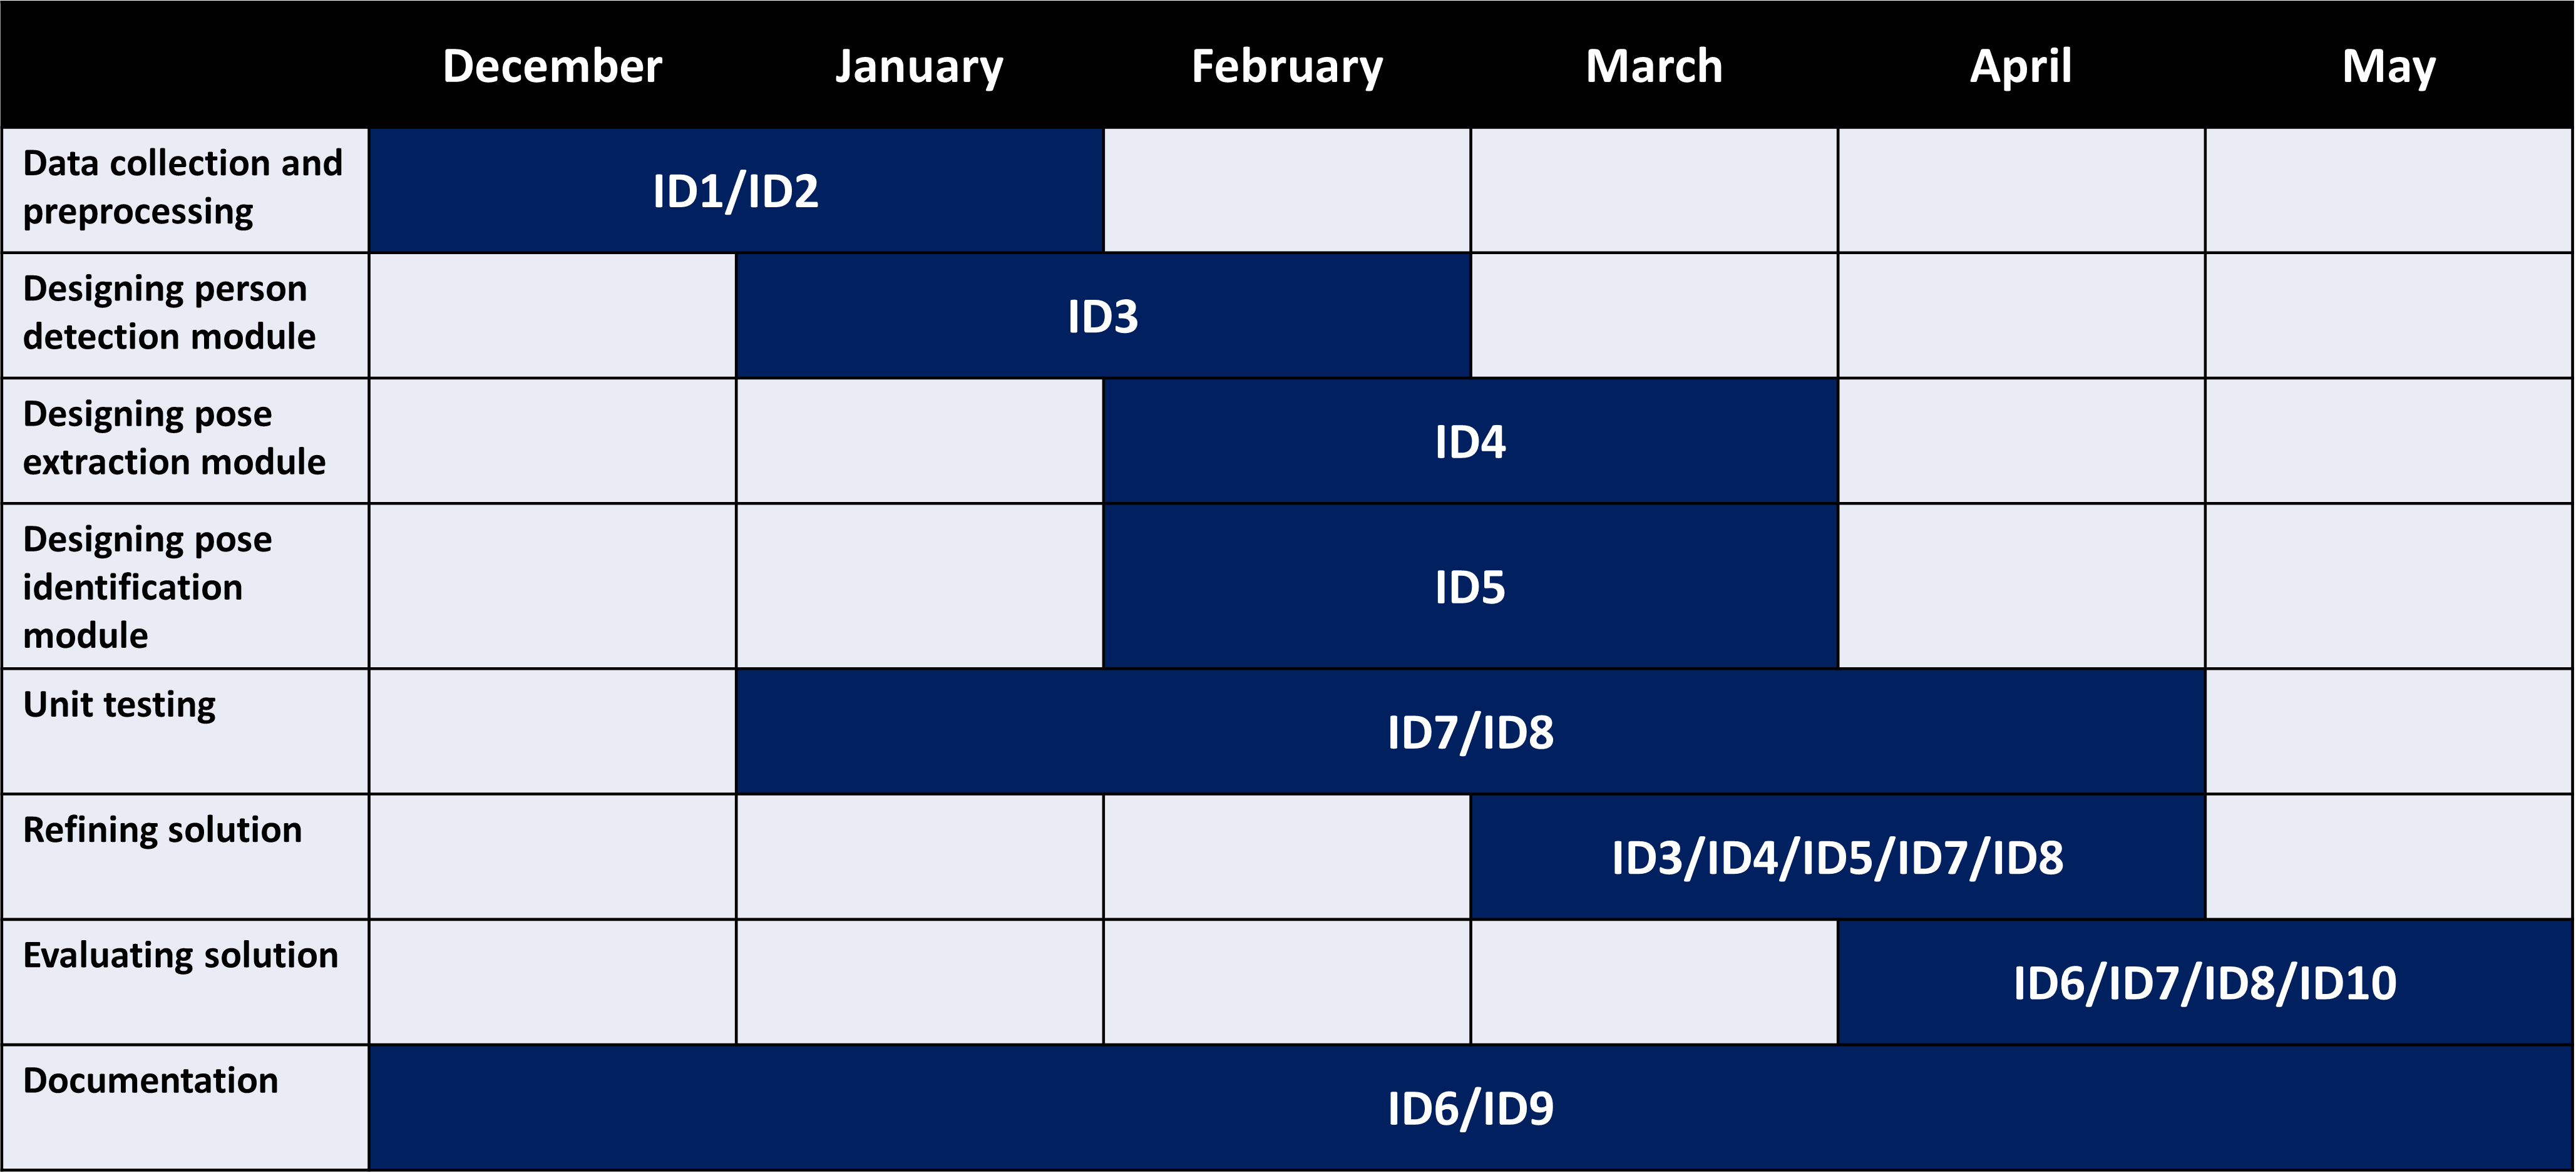
\includegraphics[scale = 0.5]{img/gantt.png}
    \caption{A GANTT chart showing the project timeline.}
    \label{fig:gantt}
\end{figure}

\subsection{Ethics, Risks and Mitigation}

Most potential ethical problems may arise from the training and use of the software - the capturing of human bio-metric and postural data. To combat this, any individual included in data recordings will be asked for their explicit consent prior to the recordings, and will be made to clearly understand what their data will be used for. If an individual does not consent, the recording will not take place. Furthermore, all personal data, images and recordings will be erased when they are no longer needed, in a way that is demonstrable and rigorous.

For the sake of diversity and inclusion, a variety of individuals will be included in recording data, so that the software is as unbiased and general as possible. People of all sexes, races, heights and sizes will be included (with their consent, in accordance with the previous paragraph).

Again, most risks specific to this project (outside general and generic risks) surround the recording of data and training of the software. If for some reason data is unable to be recorded or used, a number of backup data-sets will be employed, sourced from the internet. Only free and open-source data-sets will be used, and where such third-party data has been used, documentation will clearly state and identify said data, as well as the origin and give credit where necessary.

\section{Conclusion}

Grappling is a complex and ever-changing art, but the fundamental concept of control is always at the forefront of winning strategies. Being able to identify winning positions and understand them is the first step to becoming a better grappler, from the perspective of the teacher, referee, student or competitor.

Computer vision and deep learning have reached new heights in recent years, with new techniques, architectures and technologies constantly emerging and dominating. It is through these techniques that we can elevate our understanding of sport and competition, and the intricacies behind the best strategies and positions.

\newpage

\printbibliography

\end{document}
